\documentclass[a4paper, 12pt]{article}

% Работа с русским языком
\usepackage{cmap}
\usepackage{mathtext}
\usepackage[T2A]{fontenc}
\usepackage[utf8]{inputenc}
\usepackage[english,russian]{babel}

% Математика и графика
\usepackage{amsmath,amsfonts,amssymb,amsthm,mathtools}
\usepackage{icomma}

\usepackage{physics}
\usepackage{graphicx}
\usepackage{calc}
\usepackage{wrapfig}
\usepackage{setspace}
\usepackage{indentfirst}
\usepackage{gensymb}
\usepackage{longtable}
\usepackage{float}
\usepackage{multirow}
\setlength{\textfloatsep}{10pt}

% Точка после секции
\usepackage{titlesec}
\titlelabel{\thetitle.\quad}

\usepackage[left=25mm, top=14mm, right=25mm, bottom=30mm, nohead]{geometry}
\usepackage{fancybox,fancyhdr} 
\setcounter{page}{1} % счетчик нумерации страниц
\headsep=10mm 
\usepackage{xcolor}
\usepackage{hyperref} 
\hypersetup{colorlinks=true, allcolors=[RGB]{010 090 200}} % цвет ссылок 
\newcommand{\lr}[1]{\left({#1}\right)} % команда для скобок
\newcommand{\te}[2]{{#1}_{\text{#2}}}


\begin{document}

\begin{titlepage}
        %\setlength{\parindent}{0pt}
        %\vspace*{-3.8\baselineskip}
        \begin{center}
            %\includegraphics[width=0.2\linewidth]{logo.png}\\[1ex]
		{\large МОСКОВСКИЙ ФИЗИКО-ТЕХНИЧЕСКИЙ ИНСТИТУТ (НАЦИОНАЛЬНЫЙ ИССЛЕДОВАТЕЛЬСКИЙ УНИВЕРСИТЕТ)}
		{\large Физтех-школа физики и исследований им. Ландау}
	\end{center}
	
	
	\vspace{4.5cm}
	{\huge
		\begin{center}
			Отчет по лабораторной работе №4.4.1 \\
                \textbf{Амплитудная дифракционная решётка}\\
		\end{center}
	}
	\vspace{2cm}
	\begin{flushright} % выравнивание по правому краю
		\begin{minipage}{0.3\textwidth} % врезка в половину ширины текста
			\begin{flushleft} % выровнять её содержимое по левому краю

				\large\textbf{Работу выполнил:}\\
				\large {Комкин Михаил Валерьевич} \\
				\large {Группа: Б01-303} \\

			\end{flushleft}
		\end{minipage}
	\end{flushright}
	\vspace{8cm}
	\begin{center}
            
		Долгопрудный 2025
	\end{center}
\end{titlepage}

\textbf{Цель работы:}
Знакомство с работой и настройкой гониометра Г5,
определение спектральных характеристик амплитудной решётки. \\ 

    \textbf{В работе используется:}
гониометр, дифракционная решётка,
ртутная лампа.
\section{Теоретические сведения:}
\subsection{Принцип работы}
    Спектральными называются оптические приборы, которые осуществляют физическое 
    разложение излучения на монохроматические составляющие. По характеру распределения 
    интенсивности выделяют три вида спектров \textit{непрерывные, сплошные и линейчатые}.
    \textbf{Установка действует по следующему принципу:}
    \begin{enumerate}
        \item Свет от источника попадает на экран, которые содержит отверстие в виде щели. Экран располагают в фокальной плоскости линзы или системы линз.
        \item Коллиматор формирует пучок света, близкий к параллельному.
        \item Затем пучок лучей попадает на \textit{диспергирующий элемент} (в данной работе им является Амплитудная решетка).
        \item С помощью зрительной трубы установленной на бесконечность можно наблюдать изображение.
    \end{enumerate}



\begin{figure}[h] % h - разместить изображение здесь
    \centering
    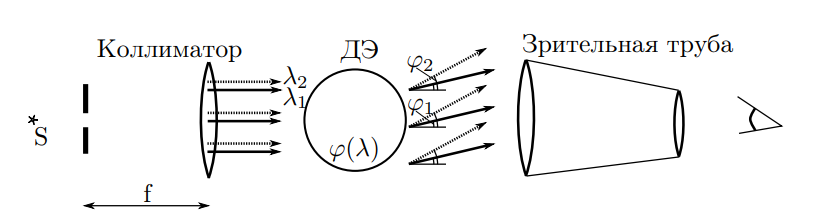
\includegraphics[width=0.7\textwidth]{ust.png} % Путь к изображению
    \caption{Схема прибора: источник-коллиматор —
    диспергирующий элемент — зрительная труба}
    \label{fig:example} % Ссылка на изображение в тексте
\end{figure}

Диспергирующий элемент пространственно разделяет монохроматические составляющие 
падающего на него излучения, осуществляя тем самым его физическое разложение по спектру. 
\textbf{Наиболее важные характеристики}
    \begin{enumerate}
        \item \textbf{Разрешающая способность} $R = \frac{\lambda}{\delta \lambda}$ характеризует возможность прибора различать две близкие спектральные линии с длинами волн $\lambda$ и $\lambda + \delta \lambda$
        \item \textbf{Угловая дисперсия} $D = \frac{d\lambda}{d \varphi}$ - производная зависимости угла отклонения $\varphi(\lambda)$ волны диспергирующим элементом по $\lambda$
        \item \textbf{Дисперсионная область} - предельная ширина спектрального интервала $\Delta \lambda$ прибора, для которой дифракционные максимумы соседних порядков не перекрываются.
    \end{enumerate}
\subsection{Амплитудная дифракционная решётка}


\begin{figure}[H] % h - разместить изображение здесь
    \centering
    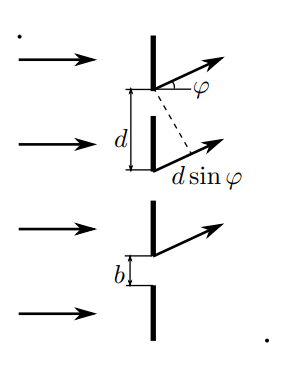
\includegraphics[width=0.3\textwidth]{diff.png} % Путь к изображению
    \caption{Дифракция
    световой волны на
    амплитудной решётке}
    \label{fig:example} % Ссылка на изображение в тексте
\end{figure}
Амплитудная решетка представляет собой непрозрачный экран, в котором прорезано $N$ параллельных щелей - штрихов. Расстояния между всеми штрихами равны $d$. 
Интенсивность дифрагированного света максимальна для углов $\varphi_m$, при которых волны, приходящие в точку наблюдения от
всех щелей, оказываются в фазе: $d sin \varphi_m = m \lambda$ ($m = 0, \pm 1, \pm 2$).

\begin{figure}[H] % h - разместить изображение здесь
    \centering
    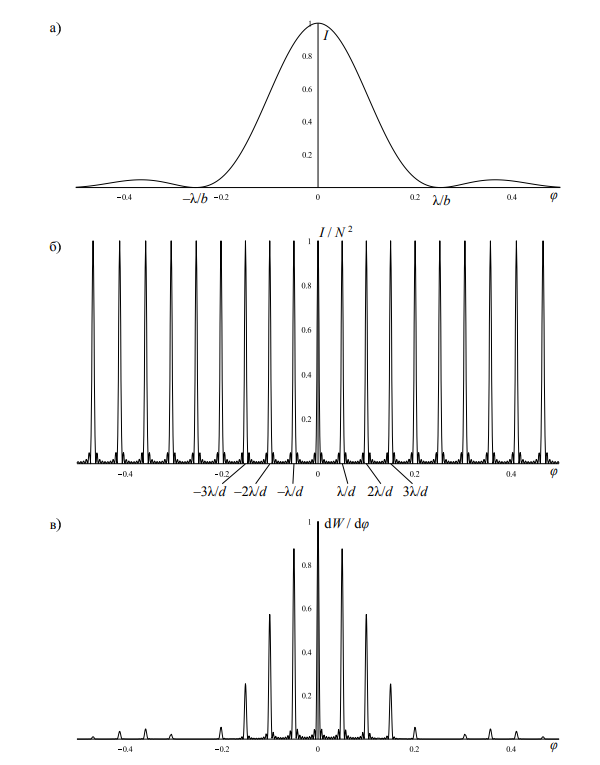
\includegraphics[width=0.7\textwidth]{diff_2.png} % Путь к изображению
    \caption{Дифракция света на решётке. Зависимость
        интенсивности света от угла: а) дифракция на отдельной щели;
        б) дифракция на решётке в пределе бесконечно узких щелей;
        в) распределение мощности света на единицу высоты изображения,
        отнесённое к малому диапазону углов}
    \label{fig:example} % Ссылка на изображение в тексте
\end{figure}


\section{Ход работы}

Сначала были измерены углы для максимумов линий спектра ртутной лампы порядков $\pm 1$. Полученные данные приведены в таблице \ref{angles}.

\begin{table}[H]
    \centering
    \begin{tabular}{|p{2cm}|p{4cm}|p{4cm}|}
    \hline  \centering{№ линии} & $\varphi_{+1}$ &  $\varphi_{-1}$ \\ \hline
$6$   & $11^{\circ} 41^{\prime} 57^{\prime \prime}$  & $11^{\circ} 38^{\prime} 29^{\prime \prime}$  \\ \hline
$5$   & $12^{\circ} 36^{\prime} 34^{\prime \prime}$  & $12^{\circ} 33^{\prime} 37^{\prime \prime}$  \\ \hline
$4$   & $14^{\circ} 15^{\prime} 39^{\prime \prime}$  & $14^{\circ} 11^{\prime} 58^{\prime \prime}$  \\ \hline
$3$   & $15^{\circ} 52^{\prime} 33^{\prime \prime}$  & $15^{\circ} 48^{\prime} 17^{\prime \prime}$  \\ \hline
$2$   & $16^{\circ} 48^{\prime}  4^{\prime \prime}$  & $16^{\circ} 43^{\prime} 18^{\prime \prime}$  \\ \hline
$1$   & $16^{\circ} 51^{\prime} 56^{\prime \prime}$  & $16^{\circ} 47^{\prime} 1^{\prime \prime}$  \\ \hline
$K_2$ & $17^{\circ} 52^{\prime}  8^{\prime \prime}$  & $17^{\circ} 47^{\prime} 11^{\prime \prime}$  \\ \hline
$K_1$ & $18^{\circ} 12^{\prime} 43^{\prime \prime}$  & $18^{\circ}  6^{\prime } 48^{\prime \prime}$  \\ \hline

        
    
    \end{tabular}
    \caption{Углы линий спектра ртути}
    \label{angles}
\end{table}


\section{Обработка данных}

По полученным данным в таблице \ref{angles} был построен график на рис.\ref{angle} зависимости $\sin \varphi_m$ от длины волны. По коэффициенту наклона c использованием формулы \eqref{main} был найден период решётки $d = \frac{1}{k} = 2,04 \pm 0,05$ мкм.

\begin{figure}[H]
    \centering
    \includegraphics[scale=0.65]{4.4.1/sin.pdf}
    \caption{График зависимости $\sin \varphi$ от длины волны для первых максимумов}
    \label{angle}
\end{figure}


\section{Вывод}

Таким образом, мы исследовали спектральные линии ртути, определили шаг решётки, её угловую дисперсию, а также её разрешающую способность. Полученные результаты близки к теоретическим вычислениям.

\end{document}